\section{Разработка принципиальной схемы}
\label{sec:principal}

\subsection{Схема питания устройства}

Как указывалось ранее блок питания содержит конденсатор емкостью 1000 мкФ и линейный стабилизатор напряжения LM7805.
Конденсатор подключается параллельно к источнику питания для сглаживания пульсаций и шумов,
обеспечивая более стабильное напряжение. Это помогает защитить чувствительный микроконтроллер 
от колебаний напряжения и улучшает общую работу устройства.

Линейный стабилизатор питается от адаптера питания 12 В и преобразует входное напряжение в 5 В\cite{LM7805_sheet}, 
нужные для питания микроконтроллера. Он также защищает схему от перепадов напряжения, шумов и пульсаций, 
а также от перегрева\cite{schemt_3}. Для защиты от перегрева самого стабилизатора на нем устанавливается радиатор. 
Изображение стабилизатора LM7805 представлено на рисунке \ref{fig:lm7805}. 
\begin{figure}[ht]
    \centering
    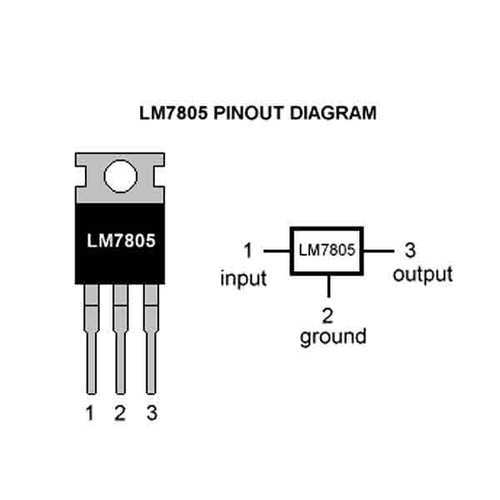
\includegraphics[width=0.4\linewidth]{\commonSecPathPrefix/sec_4/content/lm7805.jpg}
    \caption{Стабилизатор напряжения LM7805 и назначения его выводов}
    \label{fig:lm7805}
\end{figure}

\subsection{Подключение микроконтроллера}

Плата Arduino Nano подключается к устройству используя следующие выводы:

\begin{itemize}
    \item К выходу GND подключается одноименный вывод стабилизатора напряжения и исток транзистора IRZ44N;
    \item К выходу 5V подключается выходы драйверов двигателей: VCC, MS1, MS2, MS3;
    \item D11 подключается к резистору 47 Ом, который в свою очередь соединяется с затвором транзистора IRZ44N;
    \item D6 и D5 подключаются к пинам DIR обоих драйверов шаговых двигателей;
    \item D3 и D2 подключаются соответственно к пинам STEP модулей A4988.
\end{itemize}

Обозначения выводов микроконтроллера\cite{arduino_sheet} представлены на рисунке \ref{fig:arduino}.
\begin{figure}[ht]
    \centering
    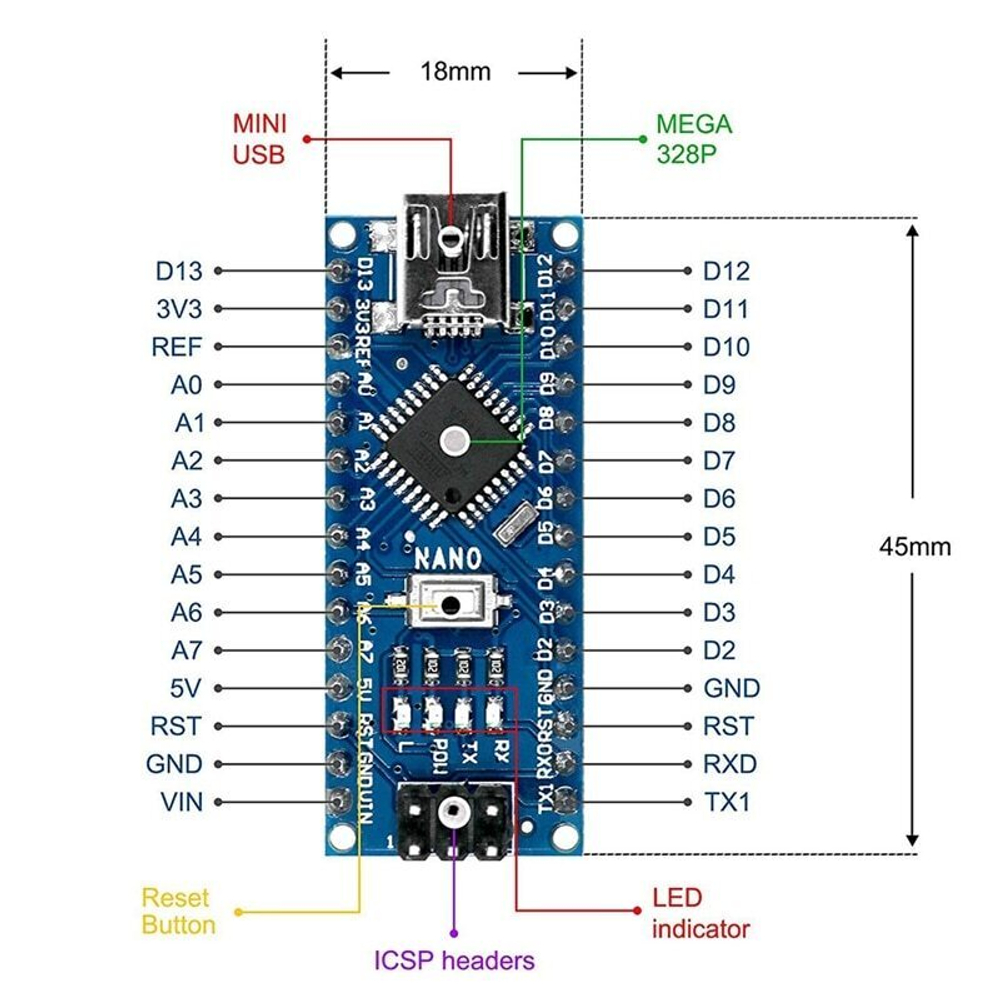
\includegraphics[width=0.6\linewidth]{\commonSecPathPrefix/sec_4/content/arduino.jpg}
    \caption{Плата Arduino Nano и обозначения ее выводов}
    \label{fig:arduino}
\end{figure}

\subsection{Подключение драйверов шаговых двигателей и моторов}

Драйвер шагового двигателя А4988 работает от напряжения 8 - 35 В и может обеспечить ток до 1 А без радиатора\cite{a4988_sheet}. 
Модуль A4988 имеет защиту от перегрузки и перегрева. 


Одним из параметров шаговых двигателей является количество шагов на один оборот (360°). 
Драйвер A4988 позволяет увеличить это значение за счет управления промежуточными шагами и поддерживает пять режимов микрошага\cite{a4988_sheet}: 
полный шаг или 1, полушаг или 1/2, 1/4, 1/8 и 1/16. Для выбора режима микрошага используются выводы MS1, MS2 и MS3 (рис. \ref{fig:a4988}). 
В таблице \ref{tab:microstepping} показано соответствие режимов микрошага и управляющих сигналов.

\begin{figure}[ht]
    \centering
    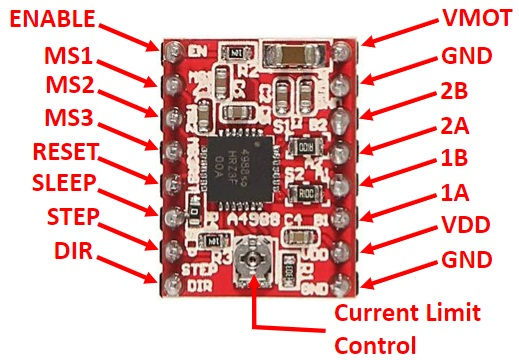
\includegraphics[width=0.4\linewidth]{\commonSecPathPrefix/sec_4/content/a4988.jpg}
    \caption{Модуль драйвера шагового двигателя A4988}
    \label{fig:a4988}
\end{figure}

\begin{table}[ht]
    \caption{Режимы микрошага драйвера A4988 и состояния выводов MS1, MS2 и MS3 по уровню напряжения}
    \centering
    \begin{tabular}{|l|l|l|l|}
        \hline
        Коэффициент дробления шага & MS1 & MS2 & MS3 \\
        \hline
        Полный шаг (1) & Низкий уровень& Низкий & Низкий \\
        \hline
        Полушаг (1/2) & Высокий уровень& Низкий & Низкий \\
        \hline
        Четверть шага (1/4) & Низкий уровень& Высокий & Низкий \\
        \hline
        Восьмая часть шага (1/8) & Высокий уровень& Высокий & Низкий \\
        \hline
        Шестнадцатая часть шага (1/16) & Высокий уровень& Высокий & Высокий \\
        \hline
    \end{tabular}
    \label{tab:microstepping}
\end{table}

Для точного управления двигателем необходимо минимизировать шаг двигателя. 
Для шага 1/16 пины MS1, MS2 и MS3 модуля A4988 подключаются друг к другу и выводятся к пину микроконтроллера 5V. 
Чтобы упростить управление и избежать случайного перехода драйвера в режим сна, выводы RESET и SLEEP соединяются вместе.

Для достижения более высоких скоростей шага, питание двигателя обычно выше, чем могло бы быть без активного ограничения тока. 
Использование шагового двигателя от DVD-привода с питанием 12 В позволяет достичь более высоких скоростей работы, 
но для предотвращения повреждения двигателя ток должен быть ограничен до 1 А. 
Для этого на драйвере A4988 используется подстроечный потенциометр.

Один из способов установки ограничения тока — перевести драйвер в режим полного шага и измерить ток, 
проходящий через одну катушку двигателя, без синхронизации входа STEP. 
Измеренный ток будет в 0,7 раза больше ограничения тока, так как обе катушки двигателя всегда включены и ограничены на 
70\% от максимального тока в режиме полного шага. Другой способ — измерить напряжение непосредственно на верхней части 
потенциометра и рассчитать результирующее ограничение тока. Ограничение тока связано с опорным напряжением следующей пропорцией: 
\[I_{max} = V_{REF} \times 1.25\]
Например, если опорное напряжение составляет 0,6 В, ограничение тока будет 0,75 А. 
Для получения тока катушки полного шага в 1 А ограничение тока должно быть:
\[1 \text{А}/ 0,7 = 1,4 \text{А};\]
что соответствует опорному напряжению 1,12 В:
\[1,4 \text{А}/ 1,25 = 1,12 \text{В}.\]

\subsection{Подключение лазера}

Как указывалось ранее, для питания лазером силы тока выходящей из пина микроконтроллера 5V недостаточно. 
Для увеличения мощности отрицательная полярность лазера (рис. \ref{fig:laser}) подключается к стоку транзистора IRFZ44N\cite{IRFZ44N_sheet}, а положительная к 
выходу стабилизатора напряжения. 

\begin{figure}[ht]
    \centering
    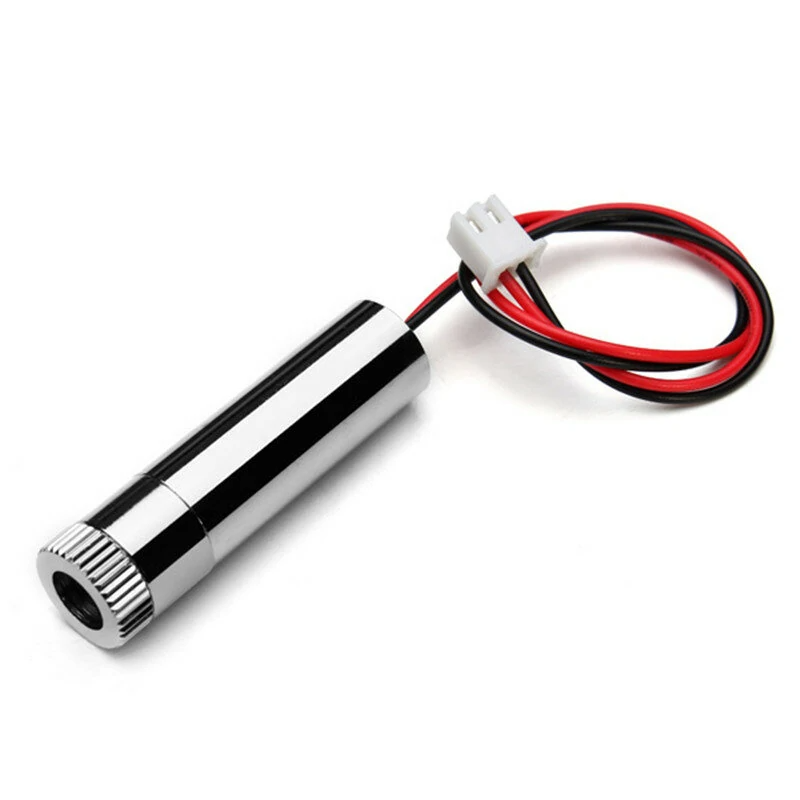
\includegraphics[width=0.4\linewidth]{\commonSecPathPrefix/sec_4/content/laser.png}
    \caption{Лазерный модуль}
    \label{fig:laser}
\end{figure}

\begin{figure}[ht]
    \centering
    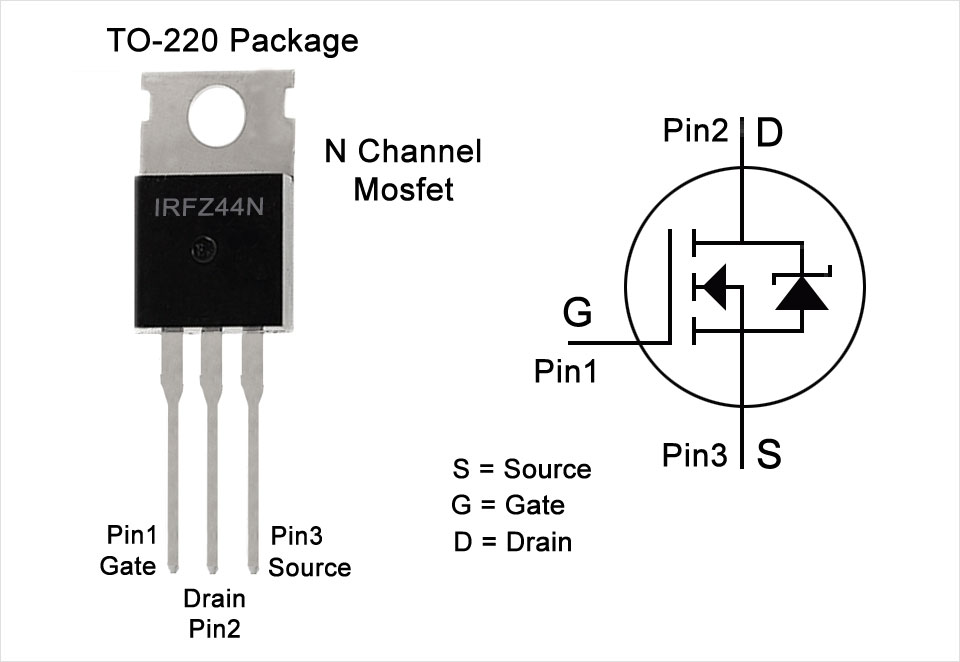
\includegraphics[width=0.5\linewidth]{\commonSecPathPrefix/sec_4/content/irfz44n.jpg}
    \caption{МОП-транзистор IRFZ44N}
    \label{fig:irfz44n}
\end{figure}

Таким образом примерная мощность лазера составляет более 1,175 Вт. Также при установке
лазера необходимо воспользоваться встроенным в него потенциометром и линзой\cite{schemt_2}.
Примерное рабочее расстояние фокусировки составляет от 5 до 8 см в зависимости от положения фокусирующей линзы.


